\documentclass[10pt,a4paper]{article}
\usepackage{amsmath}
\usepackage[utf8]{vietnam}
\usepackage{amsfonts}
\usepackage{amssymb}
\usepackage{graphicx}
\usepackage{float}
\usepackage{multicol}
\usepackage{tkz-tab}
\usepackage{colortbl}
\usepackage[left=2cm,right=2cm,top=2cm,bottom=2cm]{geometry}
\setlength{\parindent}{0pt}
\begin{document}
\fontsize{18}{30}\selectfont
{\centering TRƯỜNG ĐẠI HỌC CÔNG NGHỆ THÔNG TIN \\
KHOA KHOA HỌC MÁY TÍNH \\
BÀI TẬP MÔN PHÂN TÍCH VÀ THIẾT KẾ THUẬT TOÁN
\par}
\vspace{0.5 cm}
\begin{center}
    \begin{figure}[htp]
     \centering
\includegraphics[scale=.3]{images/logo_uit.jpg} \\
    \end{figure}
    \vspace{1 cm}
    
    \par\noindent\rule{\textwidth}{0.5pt}
    \fontsize{14}{30}\selectfont
    {\centering \textbf{HOMEWORK \#01 \\
    ĐÁNH GIÁ THUẬT TOÁN DÙNG KỸ THUẬT TOÁN SƠ CẤP} \\
    }
    \par\noindent\rule{\textwidth}{0.5pt}
    
    \fontsize{14}{30}\selectfont
    \begin{tabbing}
    \hspace{2 in} \= \hspace{2 in} \= \kill

    Môn: \> Phân tích thiết kế thuật toán \\
    Lớp: \> CS112.N23.KHCL \\
    Giảng viên hướng dẫn: \> Huỳnh Thị Thanh Thương \\
    Nhóm thực hiện: \> Hồ Thị Khánh Hiền(Leader) - 21522057 \\
    \hspace{5.3 cm}Tống Trần Tiến Dũng - 21521983 \\
    \hspace{5.3 cm}Bùi Mạnh Hùng - 21522110 \\
    \end{tabbing}  

    \begin{center}
    \fontsize{14}{30}\selectfont
     TP Hồ Chí Minh,{\today}
    \end{center}
\end{center}
\newpage
\fontsize{13}{15}\selectfont
\tableofcontents
\clearpage
\section{Tính tổng hữu hạn}
\subsection*{a)} % Dung
        \begin{equation*}
            1+3+5...+999 = \sum_{i=1}^{500}{(2i-1)}=2\sum_{i=1}^{500}{(i)}-\sum_{i=1}^{500}{(1)}=500(500+1)-500=250000
        \end{equation*}
\addcontentsline{toc}{subsection}{a)}
\subsection*{b)} % Hien
    S = 2+4+8+16+...+1024 \\
    Số hạng đầu $u_1$ = 2 \\
    Công bội q =2 \\
    \text{Có: }
        $u_{n}$ = $u_{1}q^{n-1}$
    => 1024 = 2.$2^{n-1}$ => n = 10 
    \begin{equation*}
        S = \frac{u_{1}(q^{10}-1)}{q-1} = \frac{2(2^{10}-1)}{2-1} = 2046
    \end{equation*}
\addcontentsline{toc}{subsection}{b)}
\subsection*{c)} % Hung
    \begin{equation*}
        \sum_{i=3}^{n+1}{1} = \frac{(n+1)-3+1}{2} = \frac{n-1}{2}
    \end{equation*}
\addcontentsline{toc}{subsection}{c)}
\subsection*{d)} % Dung
        \begin{equation*}
            \sum_{i=3}^{n+1}{i} = \sum_{i=1}^{n+1}{i}-\sum_{i=1}^{2}{i}=\frac{(n+1)(n+2)}{2}-3
        \end{equation*}
\addcontentsline{toc}{subsection}{d)}
\subsection*{e)} % Hien
    \begin{equation*}
        \sum_{i=0}^{n-1}{i(i+1)} = \sum_{i=0}^{n-1}{i^2}+\sum_{i=0}^{n-1}{i} 
    \end{equation*}
    \text{Đặt x = n-1 suy ra:}
    \begin{equation*}
        \sum_{i=0}^{n-1}{i^2}+\sum_{i=0}^{n-1}{i} = \sum_{i=0}^{x}{i^2}+\sum_{i=0}^{x}{i} = \frac{x(x+1)(2x+1)}{6}+\frac{x(x+1)}{2} = \frac{n(n^2-1)}{3}
    \end{equation*}
\addcontentsline{toc}{subsection}{e)}
\subsection*{f)} % Hung
    \begin{equation*}
        \sum_{j=1}^{n}3^{j+1} = 3\sum_{j=1}^{n}3^{j}=3(3^1 + 3^2 + ... + 3^n) = 3\frac{3^{n+1}-3}{2}=\frac{9}{2}(3^n-1)
    \end{equation*}
\addcontentsline{toc}{subsection}{f)}
\subsection*{g)} % Dung
    \begin{equation*}
        \sum_{i=1}^{n}{\sum_{j=1}^{n}ij} =  \sum_{i=1}^{n}i{\sum_{j=1}^{n}j}= \sum_{i=1}^{n}{i\bigg({\frac{n(n+1)}{2}}\bigg)}=\frac{n(n+1)}{2}\sum_{i=1}^{n}i=\bigg(\frac{n(n+1)}{2}\bigg)^2
    \end{equation*}
\addcontentsline{toc}{subsection}{g)}
\subsection*{h)} % Hien
    \begin{align*}
        \sum_{i=1}^{n}\frac{1}{i(i+1)}
        & = \frac{1}{1.2}+\frac{1}{2.3}+...+\frac{1}{n.(n+1)}\\ 
        & = 1-\frac{1}{2}+\frac{1}{2}-\frac{1}{3}+...+\frac{1}{n}-\frac{1}{n+1}
          =1-\frac{1}{n+1}=\frac{n}{n+1}
    \end{align*}
\addcontentsline{toc}{subsection}{h)}
\subsection*{i)} % Hung
    \begin{equation*}
        \sum_{j \in \{2,3,5\}}(j^2+j)=\sum_{j \in \{2,3,5\}}j(j+1) 
        = (2.3 + 3.4) + 5.6 = 3.6 + 5.6 = 6.8 = 48 
    \end{equation*}
\addcontentsline{toc}{subsection}{i)}
\subsection*{j)} % Dung
    \begin{equation*}
         \sum_{i=1}^{m}\sum_{j=0}^{n}{{\sum_{k=0}^{100}{(i+j)}}}=\sum_{i=1}^{m}\sum_{j=0}^{n}{{\sum_{k=0}^{100}{i}}}+\sum_{i=1}^{m}\sum_{j=0}^{n}{{\sum_{k=0}^{100}{j}}}=100n\sum_{i=1}^{m}i+100\sum_{i=1}^{m}\sum_{j=0}^{n}j    
    \end{equation*}
    \begin{equation*}
        =100n\bigg(\frac{m(m+1)}{2}\bigg)+100m\bigg(\frac{n(n+1)}{2}\bigg)
    \end{equation*}    
\addcontentsline{toc}{subsection}{j)}
\section{Tính số phép gán và so sánh}
\subsection*{Bài 2} % Hien
    \begin{figure}[H]
        \centering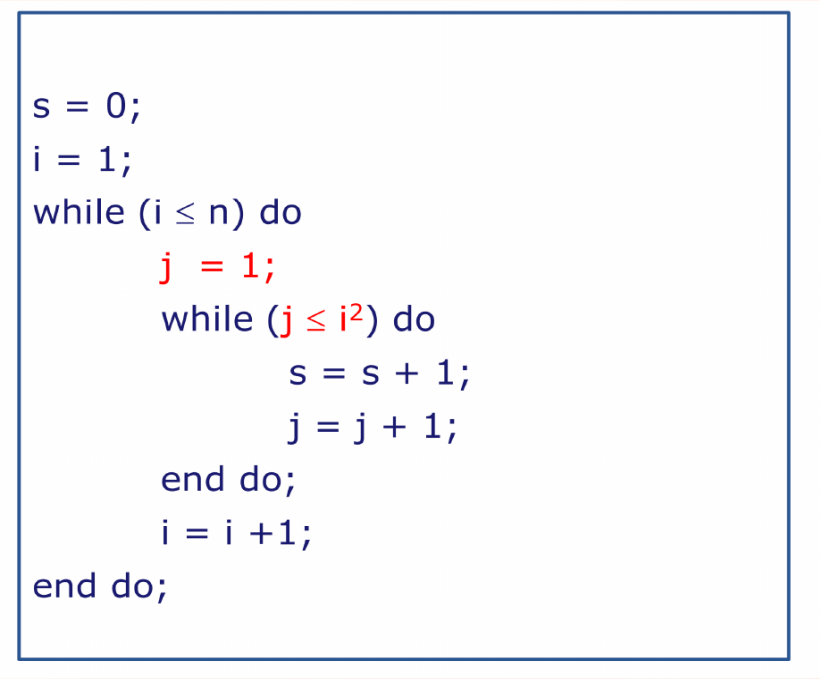
\includegraphics[scale=.6]{images/bai2.png} \\
    \end{figure}
     \textbf{Giải} \\
     Gọi $\alpha_i$ là số lần lặp của while trong = số con $j$, $j$ chạy từ 1 -> $i^2$, bước tăng là 1 = $i^2$-1+1 = $i^2$ (lần) \\
     \textbf{Kết luận}\\
     \begin{align*}
          \text{Gán(n)}
            & = 2 + 2n + \sum_{i=1}^{n}{2\alpha_i}
              = 2 + 2n + 2\sum_{i=1}^{n}{i^{2}} \\
            & = 2 + 2n + \frac{2n(n+1)(2n+1)}{6} \\
            & = 2 + 2n + \frac{n(n+1)(2n+1)}{3} \\
            & = \frac{(n+1)(2n^2+n+6)}{3}
    \end{align*}
    \begin{align*}
        \text{So sánh(n)}
            & = n + 1 + \sum_{i=1}^{n}{\alpha_i+1}
              = n + 1 + \sum_{i=1}^{n}{(i^{2}+1)} \\
            & = n + 1 + \sum_{i=1}^{n}{i^{2}} + \sum_{i=1}^{n}{1} \\
            & = n + 1 + \frac{n(n+1)(2n+1)}{6} + n \\
            & = \frac{(2n+1)(n^2+n+6)}{6} 
    \end{align*}
\addcontentsline{toc}{subsection}{Bài 2}
\subsection*{Bài 3} % Hung
    \begin{figure}[H]
        \centering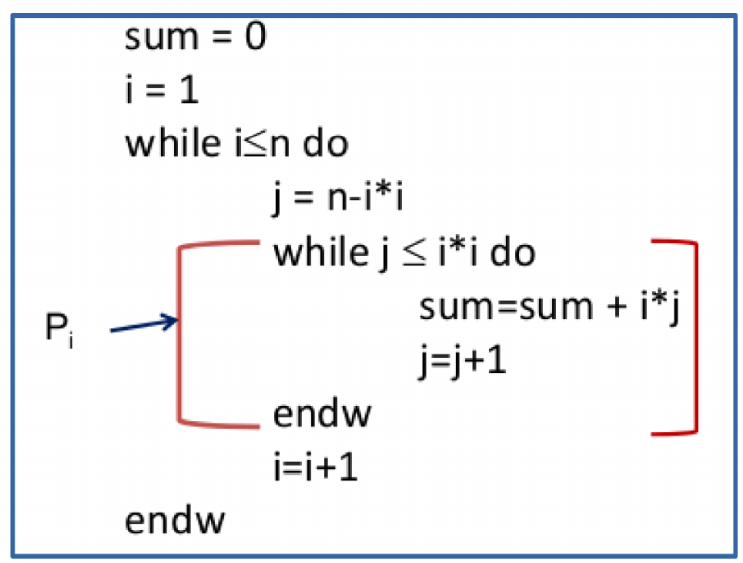
\includegraphics[scale=.6]{images/bai3.png} \\
    \end{figure} 
    \textbf{Giải} \\
    Gọi $\alpha_i$ là số lần lặp của vòng lặp While $P_i$(xét độc lập với while ngoài) \\
    Vòng lặp $P_i$ chỉ thực hiện khi $j \leq i^2 <=> n - i^2 \leq 2i^2 => i \geq \sqrt{\frac{n}{2}}(i\geq1)$ \\
    Suy ra: \\
    $
    \alpha_i = 
        \begin{cases}
            $0 , &\text{khi } i < \sqrt{\frac{n}{2}}$ \\
            $i^2-(n-i^2)+1, &\text{khi } i \geq \sqrt{\frac{n}{2}}$
        \end{cases} 
    $ \\
    \textbf{Kết luận}
    \begin{align*}
        \text{Gán(n)} 
            & = 2 + 2n + \sum_{i=1}^{n}{2\alpha_i} 
              = 2 + 2n + 2\sum_{i=\rfloor\sqrt{\frac{n}{2}}}^{n}{2i^2-n+1} \\
            & = 2 + 2n + 2(n-\rfloor\sqrt{\frac{n}{2}}+1)(1-n) + 2\sum_{i=\rfloor\sqrt{\frac{n}{2}}}^{n}{2i^2} \\
            & = 2 + 2n + 2(n-\rfloor\sqrt{\frac{n}{2}}+1)(1-n) + 
            4(\sum_{i=1}^{n}{i^2} - \sum_{i=1}^{\rfloor\sqrt{\frac{n}{2}}-1}{i^2}) \\
            & = 2 + 2n + 2(n-\rfloor\sqrt{\frac{n}{2}}+1)(1-n) + 
            4(\frac{n(n+1)(2n+1)}{6} - \frac{\alpha(\alpha+1)(2\alpha+1)}{6})
            \text{(với $\alpha = \rfloor\sqrt{\frac{n}{2}}-1$)}
    \end{align*}
    \begin{align*}
        \text{So sánh(n)}
            & = n + 1 + \sum_{i=1}^{n}{\alpha_i+1} 
              = n + 1 + n + \sum_{i=\rfloor\sqrt{\frac{n}{2}}}^{n}{2i^2-n+1} \\
            & = 2n + 1 + (n-\rfloor\sqrt{\frac{n}{2}}+1)(1-n) + \sum_{i=\rfloor\sqrt{\frac{n}{2}}}^{n}{2i^2} \\
            & = 2n + 1 + (n-\rfloor\sqrt{\frac{n}{2}}+1)(1-n) + 2(\sum_{i=1}^{n}{i^2} - \sum_{i=1}^{\rfloor\sqrt{\frac{n}{2}}-1}{i^2}) \\
            & = 2n + 1 + (n-\rfloor\sqrt{\frac{n}{2}}+1)(1-n) + \frac{n(n+1)(2n+1)-\alpha(\alpha+1)(2\alpha+1)}{3}
            \text{(với $\alpha = \rfloor\sqrt{\frac{n}{2}}-1$)}
    \end{align*}
\addcontentsline{toc}{subsection}{Bài 3}
\subsection*{Bài 4} % Dung
    \begin{figure}[H]
        \centering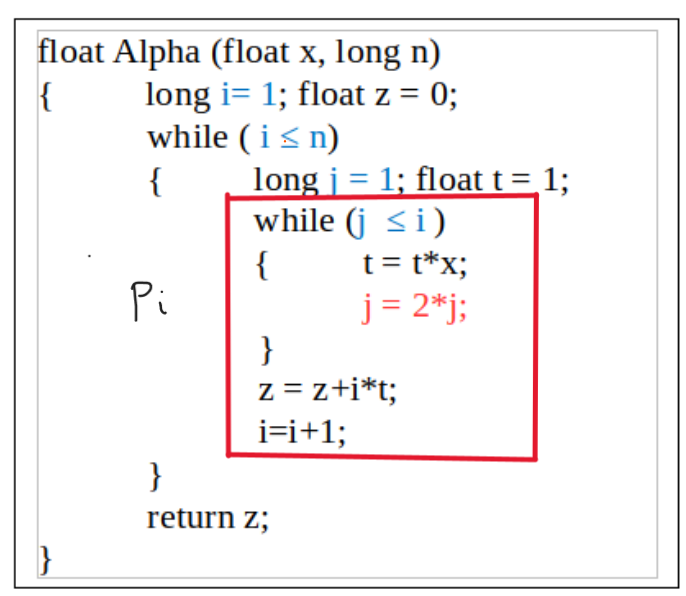
\includegraphics[scale=.6]{images/Bai4.png} \\
    \end{figure} 
    \textbf{Giải}\\
    Quy ước: Không xét câu lệnh return\\
    Số lần lặp của vòng lặp While $P_i$(xét độc lập với while ngoài): \\
    - Vòng lặp while $P_i$ chỉ thực hiện khi $j \leq i$,số lần thực hiện bằng số con j với j chạy từ 1 đến i bước tăng $2j$\\
    Gọi $\alpha_i$ là số lần lặp của $P_i$
    tập\\ $j:\{1,2,4,8,...,<=i\}$\\
    $j:\{2^0,2^1,2^2,2^3,...2^k,<=i\}$\\
    $\alpha_i = $ số con k thuộc$\{k\in N|2^k \leq i\}$
    $
        2^k \leq i\\
        \Leftrightarrow \log_2 i\leq k\\
        $mà $ k\geq 0$ $
        \rightarrow 0\leq k \leq \log_2 i\\
        \alpha_i = $ số con k $ = \log_2 i+1\\
    $
    \begin{align*}
        \text{Gán($P_i$)}
        &= 2\sum_{i=1}^{n}(\log_2 i+1) \\
        \text{So sánh($P_i$)}
        &=  \sum_{i=1}^{n}(\log_2 i+1+1)\\
        &=  \sum_{i=1}^{n}(\log_2 i+2)\\
    \end{align*}        
    \textbf{Kết luận}
    \begin{align*}
        \text{Gán(n)}
        &= 2+2+4n+2\sum_{i=1}^{n}(\log_2 i+1) \\
        &= 4+6n+2\sum_{i=1}^{n}(\log_2 i)\\
        \text{So sánh(n)}
        &= (n+1)+\sum_{i=1}^{n}(\log_2 i+2) \\
        &= 3n+1+\sum_{i=1}^{n}(\log_2 i)\\
    \end{align*}
\addcontentsline{toc}{subsection}{Bài 4}
\subsection*{Bài 5} %Hien
    \begin{figure}[H]
        \centering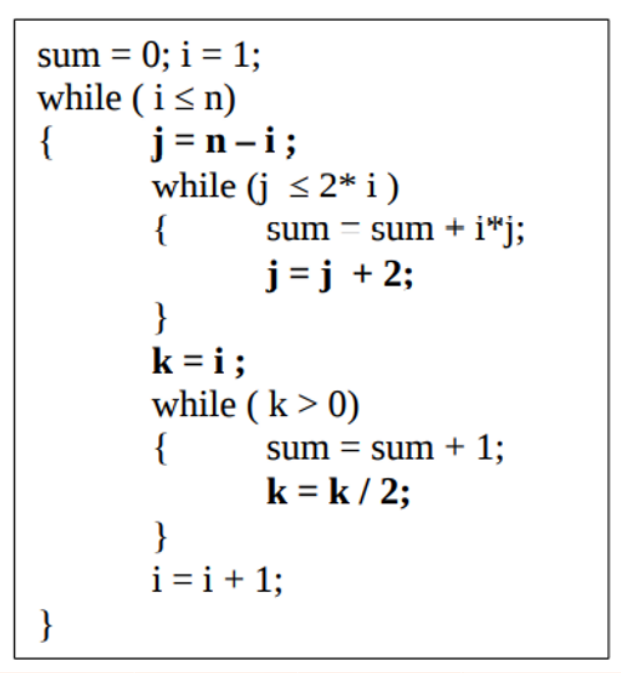
\includegraphics[scale=.7]{images/bai5.png} \\
    \end{figure}
    \textbf{Giải} \\
    Số lần lặp while ( $j \leq 2*i$)= $\alpha_i$ = số con j: n-i$\rightarrow2i$, bước tăng 2 = $\frac{2i-(n-i)}{2} + 1 = \frac{3i - n + 2}{2}$ \\
    While ( $j \leq 2*i$) chỉ thực hiện khi $n-i \leq 2i \Rightarrow i \geq \frac{n}{3}$ \\
    Suy ra: 
    $\alpha_i = 
    \begin{cases}
        (3i - n + 2)/2 &\text{khi } i \geq n/3 \\
        0 &\text{khi } i< n/3
    \end{cases}$ \\
    Số lần lặp while ($k \geq 0$) = $\beta_i$ = số con k: $i\rightarrow1$, bước giảm i/2 \\
    Tập k: \{ $\frac{i}{2^0} ,\frac{i}{2^1} ,\frac{i}{2^2} ,..,\frac{n}{2^u} \geq 1 \} \\ 
    \Rightarrow \beta_i$ là số u với \{ $u \in N | \frac{i}{2^u} \geq 1$\} \\
    $\Rightarrow i \geq 2^u \Leftrightarrow u \leq \log_2 i \Leftrightarrow 0 \leq u \leq \log_2 i$ \\
    $\Leftrightarrow \beta_i$ = số con u = $\log_2 i +1$ \\
    \textbf{Kết luận}
    \begin{align*}
          \text{Gán(n)}
            & = 2 + 3n + \sum_{i=1}^{n}{2\alpha_i} + \sum_{i=1}^{n}{2\beta_i} = 2 + 5n + \sum_{i=n/3}^{n}{(3i-n+2)} + 2\sum_{i=1}^{n}{\log_2 i} \\
            & = 2 + 5n + (2-n)(n-\frac{n}{3}+1) + \sum_{i=n/3}^{n}{3i} + 2\sum_{i=1}^{n}{\log_2 i} \\
            & = 2 + 5n +\frac{(2n+3)(2-n)}{3} + 3(\sum_{i=1}^{n}{i} - \sum_{i=1}^{\frac{n}{3}-1}{i}) + 2\sum_{i=1}^{n}{\log_2 i} \\
            & = 2 + 5n +\frac{(2n+3)(2-n)}{3} + 3\bigg(\frac{n(n+1)}{2} - \frac{\frac{n}{3}(\frac{n}{3}-1)}{2}\bigg) + 2\sum_{i=1}^{n}{\log_2 i} \\
            & = 2 + 5n + \frac{(n-1)(n-6)}{3} + 2\sum_{i=1}^{n}{\log_2 i} \\ 
            & \approx 2 + 5n + \frac{(n-1)(n-6)}{3} + 2n\log_2 n
    \end{align*}
    \begin{align*}
          \text{So sánh(n)}
            & = n + 1 + \sum_{i=1}^{n}{(\alpha_i+1)} + \sum_{i=1}^{n}{(\beta_i+1)} = 4n + 1 + \sum_{i=n/3}^{n}{\frac{3i-n+2}{2}} + \sum_{i=1}^{n}{\log_2 i} \\
            & = 4n + 1 + \frac{1}{2}\sum_{i=n/3}^{n}{(3i-n+2)} + \sum_{i=1}^{n}{\log_2 i} \\
            & = 4n + 1 + \frac{(n-1)(n-6)}{6} + \sum_{i=1}^{n}{\log_2 i} \\
            & \approx 4n + 1 + \frac{(n-1)(n-6)}{6} + n\log_2 n 
    \end{align*}
\addcontentsline{toc}{subsection}{Bài 5}
\subsection*{Bài 6} % Hung
    \begin{figure}[H]
        \centering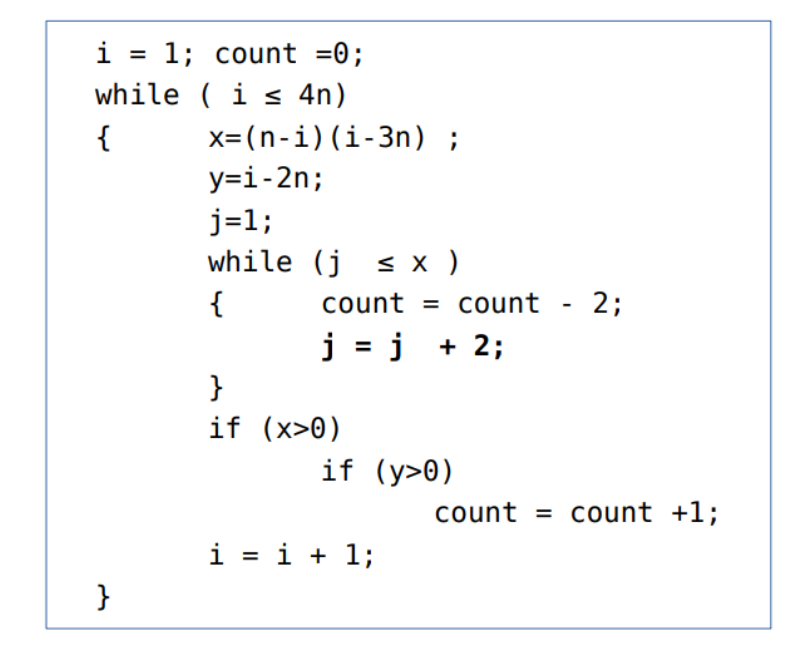
\includegraphics[scale=.6]{images/bai6.png} \\
    \end{figure} 
    \textbf{Giải} \\
    \textit{Xét bảng đổi dấu của x và y theo i} \\
    \begin{center}
    \begin{tikzpicture}    
       \tkzTabInit[lgt=3,espcl=2] 
        {$i$/1 , $x$ / 1, $y$ / 1 }
        {$1$, $n$, $2n$, $3n$, $4n$}
       \tkzTabLine { , - , 0, +, , +, 0 , - , , }
       \tkzTabLine { , - , , - , 0 , +,  , + , , }
    \end{tikzpicture} 
    \end{center}
    Câu lệnh if(y > 0) chỉ thực hiện khi (x > 0)
    \\=> Số lần thực hiện phép so sánh (y > 0) = Số con i thỏa điều kiện (x > 0) \\
    $& = (3n - 1) - (n - 1) + 1 = 2n - 1$
    \\ \\
    Câu lệnh count = count + 1 thực hiện khi (x > 0) và (y > 0)
    \\ => Số lần thực hiện phép gán (count = count + 1) 
    \\ = Số con i thỏa điều kiện (x > 0) và (y > 0)
    \\ = (3n - 1) - (2n + 1) + 1 = n - 1
    \\ \\
    Gọi $\alpha_i$ là số lần lặp của While trong $P_i$ (xét độc lập với While ngoài)
    \\ \text{Số lần lặp của While trong $P_i$ = số con j | j:1 -> x, bước tăng là 2}
    \\ Vòng lặp While trong chỉ thực hiện khi x \geq 1,hay {$ x > 0 $} => n < i < 3n
    \\ 
    $
    \alpha_i = 
        \begin{cases}
            x/2, &\text{khi } x >0 \\
            0, &\text{khi } x \leq 0
        \end{cases} 
    & = 
        \begin{cases}
            x/2, &\text{khi } n < i < 3n \\
            0, &\text{khi } i \leq n \text{ hoặc } i \geq 3n
        \end{cases}
    $ 
    \begin{align*}
         \sum_{i=1}^{4n}{\text{Gán($P_i$)}} = 
         \sum_{i=1}^{2n}{\text{2$\alpha_i$}} = 
         \sum_{i=n+1}^{3n-1}{(n-i)(i-3n)}  
    \end{align*}
    \begin{align*}
        \sum_{i=1}^{4n}{\text{So sánh($P_i$)}} = 
        \sum_{i=1}^{4n}{\text{($\alpha_i$+1)}} = 
        \sum_{i=n+1}^{3n-1}{\frac{(n-i)(i-3n)}{2}}
    \end{align*}
    \textbf{Kết luận}
    \begin{align*}
        \text{Gán(n)} 
          & = 2 + 12n + n + (n - 1) + \sum_{i=n+1}^{3n-1}{(n-i)(i-3n)} \\
          & = 14n + 1 + \sum_{i=n+1}^{3n-1}{(-i^2 + 4ni - 3n^2)} \\
          & = 14n + 1 - 3n^2[(3n-1)-(n+1)+1] + \sum_{i=n+1}^{3n-1}{(-i^2 + 4ni)} \\
          & = 14n + 1 - 3n^2(2n-1)-(\sum_{i=1}^{3n-1}{i^2}-\sum_{i=1}^{n}{i^2})
          + 4n(\sum_{i=1}^{3n-1}{i} - \sum_{i=1}^{n}{i}) \\
          & = 14n+1-6n^3+3n^2-[\frac{(3n-1)3n(6n-1)-n(n+1)(2n+1)}{6}]
          +4n[\frac{(3n-1)3n-n(n+1)}{2}] \\
          & \approx 14n+1-6n^3+3n^2 -(\frac{(3n-1)^3-n^3}{3})+4n(\frac{(3n-1)^2-n^2}{2})
    \end{align*}
    \begin{align*}
        \text{So sánh(n)}
            & = 4n+1 + 4n + 2n - 1 + \sum_{i=n+1}^{3n-1}{\frac{(n-i)(i-3n)}{2}} 
              = 10n + \sum_{i=n+1}^{3n-1}{\frac{(n-i)(i-3n)}{2}} \\
            & \approx 10n + \frac{-6n^3+3n^2 -(\frac{(3n-1)^3-n^3}{3})+4n(\frac{(3n-1)^2-n^2}{2})}{2}
    \end{align*}
\addcontentsline{toc}{subsection}{Bài 6}
\subsection*{Bài 7} % Dung
    \begin{figure}[H]
        \centering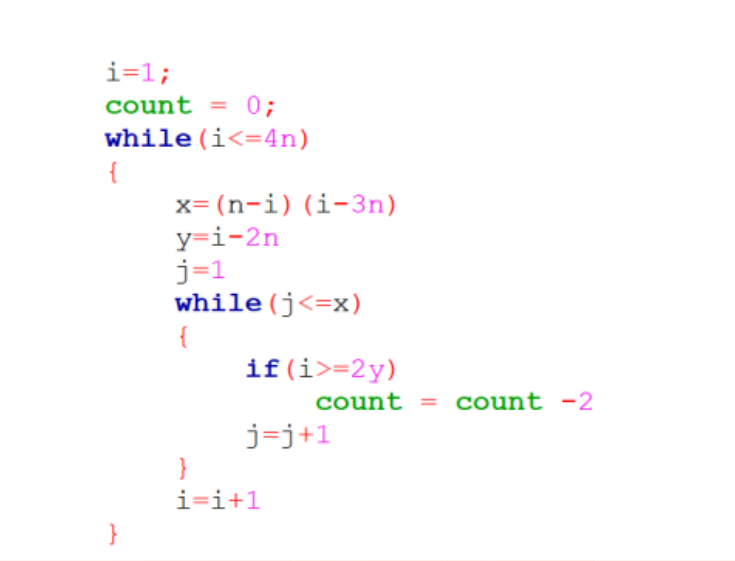
\includegraphics[scale=.6]{images/Bai7.png} \\
    \end{figure} 
    \textbf{Giải} \\
    \textit{Xét bảng đổi dấu của x theo i} \\
    \begin{center}
    \begin{tikzpicture}    
       \tkzTabInit[lgt=2,espcl=2] 
        {$i$/1 , $x$ / 1, $y$ / 1 }
        {$1$, $n$, $3n$, $4n$}
       \tkzTabLine { , - , 0, +, 0 , - , , }
    \end{tikzpicture} 
    \end{center}
    Gọi $\alpha_i$ là số lần lặp của While trong $P_i$ (xét độc lập với While ngoài)
    \\ \text{Số lần lặp của While trong $P_i$ = số con j | j:1 -> x, bước tăng là 1}
    \\ Vòng lặp While trong chỉ thực hiện khi $x \geq 1$,hay {$ x > 0 $} => $n < i < 3n$  \\ 
    $
    \alpha_i = 
        \begin{cases}
            x, &\text{khi } x >0 \\
            0, &\text{khi } x \leq 0
        \end{cases} 
        =
        \begin{cases}
            x, &\text{khi } n < i < 3n \\
            0, &\text{khi } i \leq n \text{ hoặc } i \geq 3n
        \end{cases}
    $ \\
    số lần thực hiện câu lệnh if(i$\leq$2y) = $\alpha_i$\\
    câu lệnh count = ... chỉ thực hiện khi: \\
    \begin{equation*}
        i\geq 2y
        \Leftrightarrow i \geq 2i-4n
        \Leftrightarrow i\leq 4n
    \end{equation*}        
    mà i $\leq$ 4n luôn đúng khi vòng lặp $P_i$ thực hiện\\
    $\Rightarrow$ số lần phép count = ... thực hiện = $\alpha_i$
    \begin{align*}
         \sum_{i=1}^{4n}{\text{Gán($P_i$)}} = 
         \sum_{i=1}^{4n}{\text{$\alpha_i$}}+\sum_{i=1}^{4n}{\text{$\alpha_i$}} =
         2\sum_{i=n+1}^{3n-1}{(n-i)(i-3n)}  
    \end{align*}
    \begin{align*}
        \sum_{i=1}^{4n}{\text{So sánh($P_i$)}} = 
        \sum_{i=1}^{4n}{\text{($\alpha_i$+1)}}+\sum_{i=1}^{4n}{\text{$\alpha_i$}} = 
        2\sum_{i=n+1}^{3n-1}{(n-i)(i-3n)} + \sum_{i=1}^{4n}1
    \end{align*}
    \textbf{Kết luận}
    \begin{align*}
        \text{Gán(n)} 
          & = 2 + 16n + 2\sum_{i=n+1}^{3n-1}{(n-i)(i-3n)}  \\
          & = 16n + 2 + 2\sum_{i=n+1}^{3n-1}{(n-i)(i-3n)}  \\
          & = 16n + 2 + 2\bigg[-3n^2[(3n-1)-(n+1)+1] + \sum_{i=n+1}^{3n-1}{(-i^2 + 4ni)}\bigg] \\
          & = 16n + 2 + 2\bigg[-3n^2(2n-1)-\big(\sum_{i=1}^{3n-1}{i^2}-\sum_{i=1}^{n}{i^2}\big)
          + 4n\big(\sum_{i=1}^{3n-1}{i} - \sum_{i=1}^{n}{i}\big)\bigg] \\
          & = 16n + 2 \\
          &+2\bigg[-6n^3+3n^2-\bigg(\frac{(3n-1)3n(6n-1)-n(n+1)(2n+1)}{6}\bigg)+ 4n\bigg(\frac{(3n-1)3n-n(n+1)}{2}\bigg)\bigg] \\
          & \approx 16n+2-12n^3+6n^2 -2\bigg[\frac{(3n-1)^3-n^3}{3}\bigg]+8n\bigg[\frac{(3n-1)^2-n^2}{2}\bigg]
    \end{align*}
    \begin{align*}
        \text{SS(n)}
          & = 4n+1 +  2\sum_{i=n+1}^{3n-1}{(n-i)(i-3n)} + \sum_{i=1}^{4n}1 \\
          & = 8n + 1+2\sum_{i=n+1}^{3n-1}{(n-i)(i-3n)} \\
          & = 8n + 1 + 2\bigg[-3n^2[(3n-1)-(n+1)+1] + \sum_{i=n+1}^{3n-1}{(-i^2 + 4ni)}\bigg] \\
          & = 8n + 1 + 2\bigg[-3n^2(2n-1)-\big(\sum_{i=1}^{3n-1}{i^2}-\sum_{i=1}^{n}{i^2}\big)
          + 4n\big(\sum_{i=1}^{3n-1}{i} - \sum_{i=1}^{n}{i}\big)\bigg] \\
          & = 8n + 1 \\
          &+ 2\bigg[-6n^3+3n^2-\bigg(\frac{(3n-1)3n(6n-1)-n(n+1)(2n+1)}{6}\bigg)+ 4n\bigg(\frac{(3n-1)3n-n(n+1)}{2}\bigg)\bigg] \\
          & \approx 8n+1-12n^3+6n^2 -2\bigg[\frac{(3n-1)^3-n^3}{3}\bigg]+8n\bigg[\frac{(3n-1)^2-n^2}{2}\bigg]
    \end{align*}
\addcontentsline{toc}{subsection}{Bài 7}
\subsection*{Bài 8} % Hung
    \begin{figure}[H]
        \centering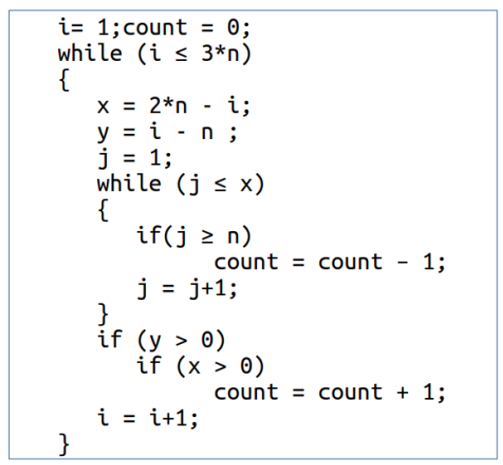
\includegraphics[scale=.7]{images/bai8.png} \\
    \end{figure} 
    \textbf{Giải} \\
    \textit{Xét bảng đổi dấu của x và y theo i} \\
    \begin{center}
    \begin{tikzpicture}    
       \tkzTabInit[lgt=3,espcl=2] 
        {$i$/1 , $x$ / 1, $y$ / 1 }
        {$1$, $n$, $2n$, $3n$}
       \tkzTabLine { , + , ,+ , 0, -,  , }
       \tkzTabLine { , - ,0 , +, , +,  , }
    \end{tikzpicture} 
    \end{center}
    Câu lệnh if(x > 0) chỉ thực hiện khi (y > 0)
    \\=> Số lần thực hiện phép so sánh (x > 0) = Số con i thỏa điều kiện (y > 0) \\
    $& = 3n - (n+1) +1 = 2n$
    \\ \\
    Câu lệnh count = count + 1 thực hiện khi (y > 0) và (x > 0)
    \\ => Số lần thực hiện phép gán (count = count + 1) 
    \\ = Số con i thỏa điều kiện (x > 0) và (y > 0)
    \\ $&= (2n-1)-(n+1)+1 = n-1 $
    \\ \\
    Gọi $\alpha_i$ là số lần lặp của While trong $P_i$ (xét độc lập với While ngoài)
    \\ \text{Số lần lặp của While trong $P_i$ = số con j | j:1 -> x, bước tăng là 1}
    \\ Vòng lặp While trong chỉ thực hiện khi x \geq 1,hay {$ x > 0 $} => $i<2n$
    \\ 
    $
    \alpha_i = 
        \begin{cases}
            0, &\text{khi } i \geq 2n\\
            x, &\text{khi } i \leq 2n-1
        \end{cases} 
    & = 
        \begin{cases}
            0, &\text{khi } i \geq 2n\\
            $2n-i$, &\text{khi } i \leq 2n-1
        \end{cases}
    $ \\ 
    \\ \text{Gọi $l_1$ là  số lần lặp của câu lệnh gán $count=count-1$}
    \\\text{Ta thấy câu lệnh gán $count=count-1$ thực hiện khi $n \leq j \leq x$} \\
    Hay,
    $
    \begin{cases}
        i \leq 2n-1 \\
        n \leq x \\
        n \leq j
    \end{cases}
    <=> 
    \begin{cases}
        i \leq 2n-1 \\
        n \leq 2n-i \\
        n \leq j
    \end{cases}
    <=>
    \begin{cases}
        i \leq 2n-1 \\
        i \leq n$ \\
        n \leq j
    \end{cases}
    &=>
    \begin{cases}
        \begin{cases}
            i \leq 2n-1\\
            n \leq j
        \end{cases}, &\text{khi } n<1 \\
        \begin{cases}
            i \leq n\\
            n \leq j
        \end{cases}, &\text{khi } n\geq1 \\
    \end{cases}
    $ \\
    \\
    \textbf{Kết luận} \\
    \textbf{\textit{Trường hợp: $n\geq1$}}
    \begin{align*}
        \text{Gán(n)} 
          & =2 + 9n + (n-1) + 3n + \sum_{i=1}^{3n}{[\alpha_i+ (x-n+1)]} \\
          & =13n + 1 + \sum_{i=1}^{2n-1}{(2n-i)} + \sum_{i=1}^{n}{(n-i+1)} \\
          & =13n + 1 + 2n(2n-1) - \sum_{i=1}^{2n-1}{i} + n(n+1) - \sum_{i=1}^{n}{i} \\
          & = 13n + 1 + 4n^2-2n - \frac{(2n-1+1)(2n-1)}{2} + n^2+n - \frac{n(n+1)}{2} \\
          & = 5n^2 + 12n + 1 - \frac{2n(2n-1)+n(n+1)}{2} = 5n^2 + 12n + 1 - \frac{5n^2-n}{2}
    \end{align*}
    \begin{align*}
        \text{So sánh(n)}
            & = (3n+1) + \sum_{i=1}^{3n}{(\alpha_i+1)} +\sum_{i=1}^{i=3n}{\alpha_i} + (3n) + [3n-(n+1)+1] \\
            & = 11n+1 + 2\sum_{i=1}^{2n-1}{2n-i} = 11n+1 + 4n(2n-1) - 2\sum_{i=1}^{2n-1}{i}\\
            & = 8n^2+1 + 7n - 2\frac{(2n-1+1)(2n-1)}{2} = 8n^2+1 + 7n - 4n^2+2n=4n^2+9n+1
    \end{align*}
    \textbf{\textit{Trường hợp: $n<1$}}
    \begin{align*}
        \text{Gán(n)} 
          & = 2
    \end{align*}
    \begin{align*}
        \text{So sánh(n)}
          & = 1
    \end{align*}
\addcontentsline{toc}{subsection}{Bài 8}
\subsection*{Bài 9} %Hien
    \begin{figure}[H]
        \centering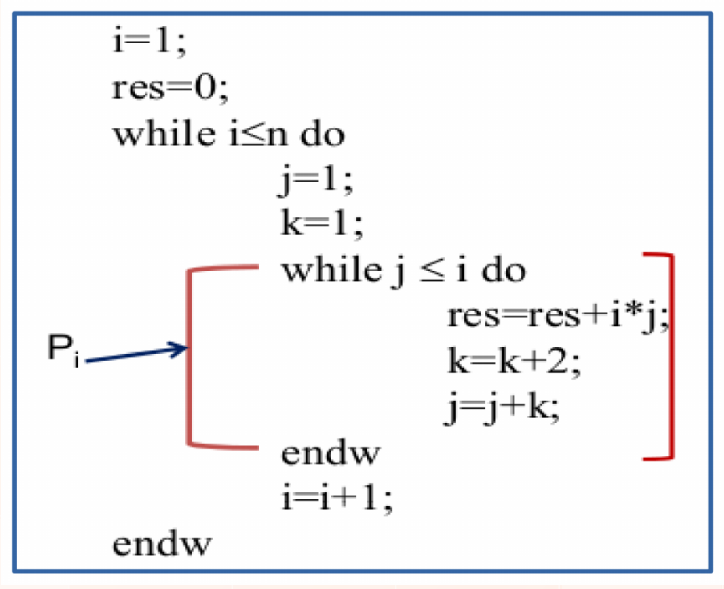
\includegraphics[scale=.6]{images/bai9.png} \\
    \end{figure}
    \textbf{Giải} \\
     Gọi $\alpha_i$ là số lần lặp của while trong \\
     Tại j = j+k, ta thấy j luôn là tổng của các số 1,3,5,7,... => j thuộc tập hợp các số chính phương. \\
     \textit{Chứng minh j luôn là số chính phương:} j=1+3+5+...+x \\
     Đặt x = 2y-1 ($y\in N$, y>1) 
     \begin{align*}
         j = 1+3+5+...+2y-1 = \frac{(2y-1)+1}{2} \bigg(\frac{(2y-1)-1}{2}+1\bigg) = y^{2}
     \end{align*}
     => điều cần chứng minh\\
     $\alpha_i$ là số con t với \{$t\in N$ | t \geq 1 , $t^{2}$ \leq i\} => \begin{cases}
            t \geq 1 \\
            -\sqrt{i} \leq t \leq \sqrt{i}
        \end{cases}  
    => $1 \leq t \leq \sqrt{i}$ \\
    => $\alpha_i$ = $\sqrt{i}$ \\
     \textbf{Kết luận}
     \begin{align*}
        \text{Gán(n)}
        & = 2 + 3n + \sum_{i=1}^{n}{3\alpha_i} = 2 + 3n + 3\sum_{i=1}^{n}{i^{1/2}} \\
        & \approx 2 + 3n + \frac{3n^{\frac{1}{2}+1}}{\frac{1}{2}+1} = 2 + 3n + 2n^{3/2}
     \end{align*}
     \begin{align*}
        \text{So sánh(n)}
        & = n + 1 + \sum_{i=1}^{n}{\alpha_i+1} = 2n + 1 + \sum_{i=1}^{n}{i^{1/2}} \\
        & \approx 2n + 1 + \frac{n^{\frac{1}{2}+1}}{\frac{1}{2}+1} = 2n + 1 + \frac{2}{3}n^{3/2}
     \end{align*}
\addcontentsline{toc}{subsection}{Bài 9}
\subsection*{Bài 10} %Hung
    \begin{figure}[H]
        \centering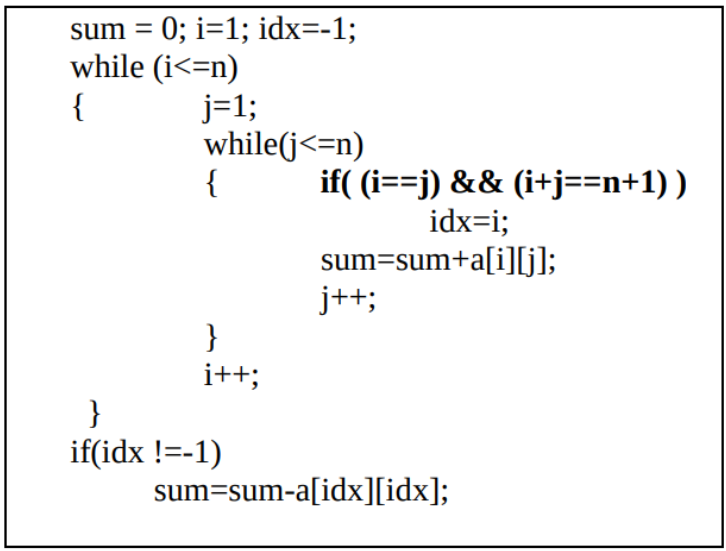
\includegraphics[scale=.6]{images/bai10.png} \\
    \end{figure} 
    \textbf{Giải} \\
    % n chan
    \textbf{Xét TH: n là số chẵn} \\
    \text{Xét vòng lặp While trong, ta thấy:}
    \begin{itemize}
        \item Câu lệnh $if((i==j)\&\&(i+j==n+1))$ đúng <=> $2i = n+1 | i\in N$ 
        \\ Mà n chẵn => không có i thỏa mãn
        \\ => Câu lệnh gán (idx=i) thực hiện 0 lần
        \item Số lần thực hiện lệnh so sánh (i+j==n+1) \\
        &  = Số lần câu lệnh so sánh (i==j) đúng = 1 lần
    \end{itemize}
    \begin{align*}
         \sum_{i=1}^{n}{\text{Gán($P_i$)}}
         = \sum_{i=1}^{n}{2} = 2n
    \end{align*}
    \begin{align*}
        \sum_{i=1}^{n}{\text{So sánh($P_i$)}} = 
        \sum_{i=1}^{n}{n+1+n + 1} = \sum_{i=1}^{n}{2n+2} = 2n^2+2n
    \end{align*}
    \textbf{Vậy}
    \begin{align*}
        \text{Gán(n|n chẵn)} 
          & = 3 + 2n + 2n = 4n + 3
    \end{align*}
    \begin{align*}
        \text{So sánh(n|n chẵn)}
            & = n+1+2n^2+2n+1 = 2n^2+3n+2
    \end{align*}
    % n le
    \textbf{Xét TH: n là số lẻ} \\
    \text{Xét vòng lặp While trong, ta thấy:}
    \begin{itemize}
        \item Câu lệnh $if((i==j)\&\&(i+j==n+1))$ đúng <=> $2i = n+1 | i\in N$ 
        \\ Mà n lẻ => có 1 giá trị i = (n+1)/2 thỏa mãn
        \\ => Câu lệnh gán (idx=i) thực hiện 1 lần khi i = (n+1)/2
        \item Số lần thực hiện lệnh so sánh (i+j==n+1) \\&= Số lần câu lệnh so sánh (i==j) đúng = 1 lần
    \end{itemize}
    \begin{align*}
         \sum_{i=1}^{n}{\text{Gán($P_i$)}}
         = 1+ \sum_{i=1}^{n}{2} = 2n + 1
    \end{align*}
    \begin{align*}
        \sum_{i=1}^{n}{\text{So sánh($P_i$)}} = 
        \sum_{i=1}^{n}{n+1+n + 1} = \sum_{i=1}^{n}{2n+2} = 2n^2+2n
    \end{align*}
    \textbf{Vậy}
    \begin{align*}
        \text{Gán(n|n lẻ)} 
          & = 3 + 2n + 2n + 1 +1 =4n+5
    \end{align*}
    \begin{align*}
        \text{So sánh(n|n lẻ)}
            & = n+1 + 2n^2+2n + 1 = 2n^2 + 3n+2
    \end{align*}
\addcontentsline{toc}{subsection}{Bài 10}
\section{[BONUS]Tính số phép gán và so sánh \& kiểm tra kết quả đếm bằng máy tính}
\subsection*{Bài 11} %Dung
    \begin{figure}[H]
        \centering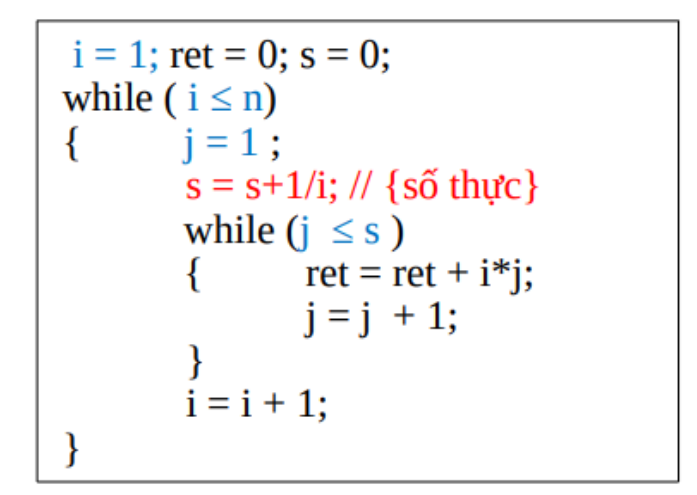
\includegraphics[scale=.6]{images/Bai11.png} \\
    \end{figure}
    \textbf{Giải} \\
     Gọi $\alpha_i$ là số lần lặp của While trong $P_i$ (xét độc lập với While ngoài)
    \\ \text{Số lần lặp của While trong $P_i$ = số con j | j:1 -> s, bước tăng là 1}\\
    \begin{align*}
        s =  \sum_{j=0}^{i}\frac{1}{j}
    \end{align*}
    vì s là số thực, suy ra: với mỗi con i, số con j thoã mãn điều kiện j$\leq$s  là phần nguyên của s:\\
    \begin{align*}
        \Leftrightarrow \alpha_i = \big[\sum_{j=0}^{i}\frac{1}{j}\big]
    \end{align*}
    \begin{align*}
        \text{Gán($P_i$)}
        & = 2\sum_{i=1}^{n}\big[\alpha_i\big]\\
        \text{So sánh($P_i$)}
        & = \sum_{i=1}^{n}\big[\alpha_i+1\big]
    \end{align*}
    \textbf{Kết luận}
    \begin{align*}
        \text{Gán(n)}
        & = 3 + 3n + 2\sum_{i=1}^{n}\big[\alpha_i\big]\\
        & = 3 + 3n + 2\sum_{i=1}^{n}\big[\sum_{j=0}^{i}\frac{1}{j}\big]\\
        & \approx 3 + 3n + 2\sum_{i=1}^{n}\big[\ln{i}+ \gamma\big] (\text{với} \gamma \approx 0.5772)\\
    \end{align*}
    \begin{align*}
        \text{So sánh(n)}
        & = (n+1) + \sum_{i=1}^{n}\big[\alpha_i+1\big]\\
        & = (n+1) + \sum_{i=1}^{n}\big(\big[\alpha_i\big]+1\big)\\
        & = (n+1) + \sum_{i=1}^{n}\big[\sum_{j=0}^{i}\frac{1}{j}\big]+\sum_{i=1}^{n}1\\
        & \approx 2n+1 + \sum_{i=1}^{n}\big[\ln{i}+ \gamma\big](\text{với} \gamma \approx 0.5772)\\  
    \end{align*}
    \textbf{Bảng so sánh kết quả giữa công thức thủ công và chạy chương trình: }
    \fontsize{12}{14}\selectfont
    \renewcommand{\arraystretch}{2}
    \setlength{\arrayrulewidth}{1pt}
    \arrayrulecolor{blue}
    \begin{table}[H]
        \centering
        \begin{tabular} [c]{|p{5cm}|p{0.75cm}|p{0.75cm}|p{0.75cm}|p{0.75cm}|p{0.75cm}|p{0.75cm}|p{0.75cm}|p{0.75cm}|p{0.75cm}|p{0.75cm}|}
        \hline
        \rowcolor[rgb]{0, .60, .800}
        n & 1 & 2 & 3 & 4 & 5 & 6 & 7 & 8 & 9 & 10 \\
        \hline
        G(n) = $3 + 3n + 2\sum_{i=1}^{n}\big[\ln{i}+ \gamma\big]$ & 6 & 11 & 16 & 21 & 28 & 35 & 42 & 48 & 56 & 63  \\
        \hline
        \rowcolor[rgb]{0, .60, .800}
        G(n) khi chạy chương trình = & 8 & 13 & 18 & 25 & 32 & 39 & 46 & 53 & 60 & 67 \\
        \hline 
        SS(n) = $2n+1 + \sum_{i=1}^{n}\big[\ln{i}+ \gamma\big]$ & 3 & 6 & 9 & 12 & 16 & 20 & 24 & 28 & 32 & 36 \\
        \hline
        \rowcolor[rgb]{0, .60, .800}
        SS(n) khi chạy chương trình = & 4 & 7 & 10 & 14 & 18 & 22 & 26 & 30 & 34 & 38 \\
        \hline
    \end{tabular}
    \end{table}
    \begin{table}[H]
        \centering
        \begin{tabular} [c]{|p{5cm}|p{0.75cm}|p{0.75cm}|p{0.75cm}|p{0.75cm}|p{0.75cm}|p{0.75cm}|p{0.75cm}|p{0.75cm}|p{0.75cm}|p{0.75cm}|}
        \hline
        \rowcolor[rgb]{0, .60, .800}
        n & 11 & 12 & 13 & 14 & 15 & 16 & 17 & 18 & 19 & 20 \\
        \hline
        G(n) = $3 + 3n + 2\sum_{i=1}^{n}\big[\ln{i}+ \gamma\big]$ & 70 & 76 & 85 & 97 & 106 & 115 & 124 & 135 & 142 & 151  \\
        \hline
        \rowcolor[rgb]{0, .60, .800}
        G(n) khi chạy chương trình = & 76 & 85 & 94 & 103 & 112 & 121 & 130 & 139 & 148 & 157 \\
        \hline 
        SS(n) = $2n+1 + \sum_{i=1}^{n}\big[\ln{i}+ \gamma\big]$ & 40 & 45 & 50 & 55 & 60 & 65 & 70 & 75 & 80 & 85 \\
        \hline
        \rowcolor[rgb]{0, .60, .800}
        SS(n) khi chạy chương trình = & 43 & 48 & 53 & 58 & 63 & 68 & 73 & 78 & 83 & 88 \\
        \hline
    \end{tabular}
    \end{table}
\addcontentsline{toc}{subsection}{Bài 11}
\subsection*{Bài 12} %Hien
    \begin{figure}[H]
        \centering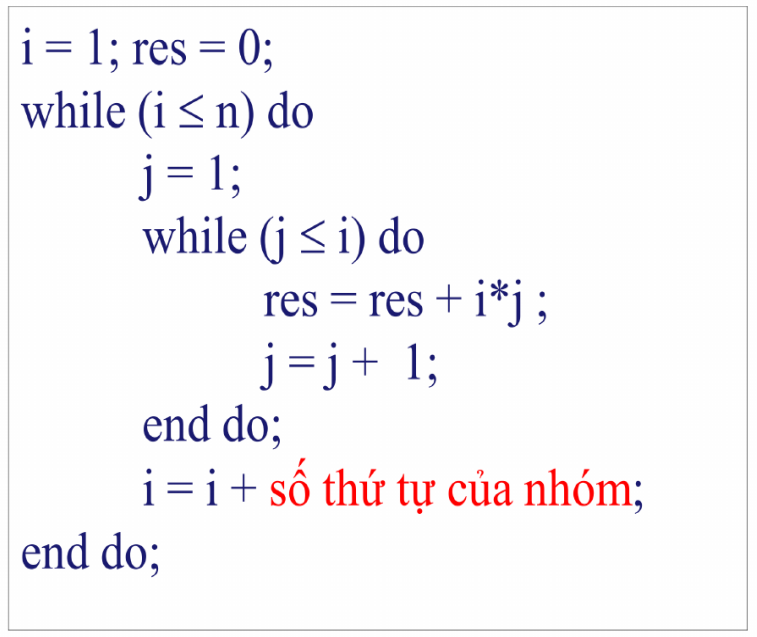
\includegraphics[scale=.6]{images/bai12.png} \\
    \end{figure}
    \textbf{Giải} \\
    Số lần lặp while ngoài = số con i chạy từ 1 -> n, bước tăng 7 = [$\frac{n-1}{7}$ + 1] = [$\frac{n+6}{7}$] (lần) \\
    Số lần lặp while trong = x = số con j chạy từ: 1 -> i, bước tăng 1. \\
    Vì bước tăng của i là 7 $\Rightarrow$ i có dạng: $7k+1, k \in N$ \\
    Có: $i \leq n \Rightarrow 7k+1 \leq n \Rightarrow k \leq [\frac{n-1}{7}]$ \\
    $\Rightarrow x = 7k+1$ với k $\in N, 0 \leq k \leq [\frac{n-1}{7}]$\\
    \textbf{Kết luận}
    \begin{align*}
        \text{Gán(n)}
        & = 2 + 2\big[\frac{n+6}{7}\big] + \sum_{k=0}^{[\frac{n-1}{7}]}{2x} \\
        & = 2 + 2\big[\frac{n+6}{7}\big] + 2\sum_{k=0}^{[\frac{n-1}{7}]}{(7k+1)}\\
        & = 2 + 2(y+1) + 14\sum_{k=0}^{y}{k} + \sum_{k=0}^{y}{2} \
        \text{(với y = $\big[\frac{n-1}{7}\big]$) } \\
        & = 4 + 2y + 7y(y+1) + 2(y+1) \\
        & = 7y^2 + 11y + 6 = 7\big[\frac{n-1}{7}\big]^2 + 11\big[\frac{n-1}{7}\big] + 6
    \end{align*}
    \begin{align*}
        \text{So sánh(n)}
        & = \big[\frac{n+6}{7}\big] + 1 + \sum_{k=0}^{[\frac{n-1}{7}]}{(x+1)} \\
        & = \big[\frac{n+6}{7}\big] + 1 + \sum_{k=0}^{[\frac{n-1}{7}]}{(7k+2)} \\
        & = y+2 + 7\sum_{k=0}^{y}{k} + \sum_{k=0}^{y}{2} \
        \text{(với y = $\big[\frac{n-1}{7}\big]$) } \\
        & = y + 2 + \frac{7y(y+1)}{2} + 2(y+1) \\
        & = \frac{7y^2 + 13y + 8}{2} = \frac{7\big[\frac{n-1}{7}\big]^2 + 13\big[\frac{n-1}{7}\big]+8}{2}
    \end{align*}
    \textbf{Bảng so sánh kết quả giữa công thức thủ công và chạy chương trình: }
    \fontsize{12}{14}\selectfont
    \renewcommand{\arraystretch}{2}
    \setlength{\arrayrulewidth}{1pt}
    \arrayrulecolor{blue}
    \begin{table}[H]
        \centering
        \begin{tabular} [c]{|p{5cm}|p{0.75cm}|p{0.75cm}|p{0.75cm}|p{0.75cm}|p{0.75cm}|p{0.75cm}|p{0.75cm}|p{0.75cm}|p{0.75cm}|p{0.75cm}|}
        \hline
        \rowcolor[rgb]{0, .60, .800}
        n & 1 & 2 & 3 & 4 & 5 & 6 & 7 & 8 & 9 & 10 \\
        \hline
        G(n) = $7\big[\frac{n-1}{7}\big]^2 + 11\big[\frac{n-1}{7}\big]$ + 6 & 6 & 6 & 6 & 6 & 6 & 6 & 6 & 24 & 24 & 24  \\
        \hline
        \rowcolor[rgb]{0, .60, .800}
        G(n) khi chạy chương trình = & 6 & 6 & 6 & 6 & 6 & 6 & 6 & 24 & 24 & 24 \\
        \hline 
        SS(n) = $\frac{7\big[\frac{n-1}{7}\big]^2 + 13\big[\frac{n-1}{7}\big]+8}{2}$ & 4 & 4 & 4 & 4 & 4 & 4 & 4 & 14 & 14 & 14 \\
        \hline
        \rowcolor[rgb]{0, .60, .800}
        SS(n) khi chạy chương trình = & 4 & 4 & 4 & 4 & 4 & 4 & 4 & 14 & 14 & 14 \\
        \hline
    \end{tabular}
    \end{table}
    \begin{table}[H]
        \centering
        \begin{tabular} [c]{|p{5cm}|p{0.75cm}|p{0.75cm}|p{0.75cm}|p{0.75cm}|p{0.75cm}|p{0.75cm}|p{0.75cm}|p{0.75cm}|p{0.75cm}|p{0.75cm}|}
        \hline
        \rowcolor[rgb]{0, .60, .800}
        n & 11 & 12 & 13 & 14 & 15 & 16 & 17 & 18 & 19 & 20 \\
        \hline
        G(n) = $7\big[\frac{n-1}{7}\big]^2 + 11\big[\frac{n-1}{7}\big]$ + 6 & 24 & 24 & 24 & 24 & 56 & 56 & 56 & 56 & 56 & 56  \\
        \hline
        \rowcolor[rgb]{0, .60, .800}
        G(n) khi chạy chương trình = & 24 & 24 & 24 & 24 & 56 & 56 & 56 & 56 & 56 & 56 \\
        \hline 
        SS(n) = $\frac{7\big[\frac{n-1}{7}\big]^2 + 13\big[\frac{n-1}{7}\big]+8}{2}$ & 14 & 14 & 14 & 14 & 31 & 31 & 31 & 31 & 31 & 31 \\
        \hline
        \rowcolor[rgb]{0, .60, .800}
        SS(n) khi chạy chương trình = & 14 & 14 & 14 & 14 & 31 & 31 & 31 & 31 & 31 & 31 \\
        \hline
    \end{tabular}
    \end{table}
\addcontentsline{toc}{subsection}{Bài 12}
\subsection*{Bài 13} %Hung
    \begin{figure}[H]
        \centering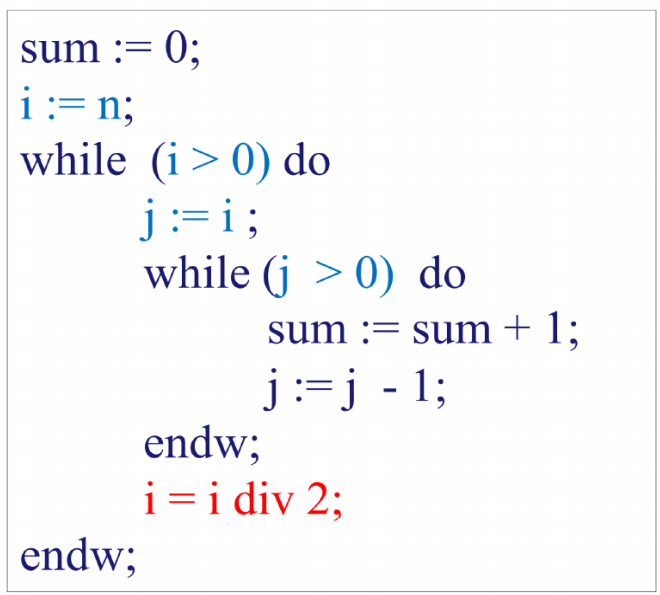
\includegraphics[scale=.7]{images/bai13.png} \\
    \end{figure} 
    \textbf{Giải} \\
    Số lần lặp của While ngoài = Số con i chạy từ i:n->1,bước giảm i/2 \\
    Ta thấy: i = \{ $\frac{n}{2^0}$ ,$\frac{n}{2^1}$ ,$\frac{n}{2^2}$ ,..,$\frac{n}{2^k}$ \} \\
    $i > 0 <=> \frac{n}{2^k} \geq 1 <=> n \geq 2^k <=> k \leq \log_2 n$ \\
    \text{$\alpha_i$ = số con k},0 \leq k \leq $\log_2 n$ => \alpha_i = $\log_2 n$ +1 \\
    \textbf{Kết luận}
    \begin{align*}
        \text{Gán(n)} 
          & = \sum_{k=0}^{\rfloor\log_2 n}{(2+\sum_{j=1}^{\frac{n}{2^k}}{2})} + 2 
            = \sum_{k=0}^{\rfloor\log_2 n}2 + \sum_{k=0}^{\rfloor\log_2 n}(\sum_{j=1}^{\frac{n}{2^k}}{2}) + 2 
            \approx 2(\rfloor\log_2 n +1) + 2n\sum_{k=0}^{\rfloor\log_2 n}{\frac{1}{2^k}} + 2 \\
          & \approx 2(\rfloor\log_2 n) + 4 + 2n(1+ \frac{1}{2} + \frac{1}{2^2}+...+\frac{1}{2^(\rfloor\log_2 n)})
    \end{align*}
    \begin{align*}
        \text{So sánh(n)}
            & = \alpha_i +1 + \sum_{k=0}^{\log_2 n}{(\sum_{j=1}^{\frac{n}{2^k}}{1} + 1)} = \log_2 n + 2 + \sum_{k=0}^{\log_2 n}{(\sum_{j=1}^{\frac{n}{2^k}}{1} + 1)} \\
            & \approx \rfloor\log_2 n + 2 + \sum_{k=0}^{\log_2 n}{(\sum_{j=1}^{\frac{n}{2^k}}{1})} + \rfloor\log_2 n + 1 \approx \rfloor\log_2 n + 2 + \sum_{k=0}^{\log_2 n}{\rfloor\frac{n}{2^k}} + \rfloor\log_2 n + 1 \\
            & \approx 2\rfloor\log_2 n + 3 +  \sum_{k=0}^{\log_2 n}{\rfloor\frac{n}{2^k}}
    \end{align*}
    \newpage
    \centering\textbf{Bảng so sánh kết quả giữa công thức thủ công và chạy chương trình: }
    \fontsize{12}{14}\selectfont
    \renewcommand{\arraystretch}{1.5}
    \setlength{\arrayrulewidth}{1pt}
    \arrayrulecolor{blue}
    \begin{table}[h]
        \centering
        \begin{tabular}[c]
        {|p{2.5cm}|p{1cm}|p{1cm}|p{1cm}|p{1cm}|p{1cm}|p{1cm}|p{1cm}|p{1cm}|p{1cm}|p{1cm}|p{1cm}|}\hline
            \rowcolor[rgb]{0, .60, .800}n&1&2&3&4&5&6&7&8&9&10\tabularnewline\hline
            G(n)-(a)  & 6 & 10 & 12 & 16 & 18 & 20 & 22 & 26 & 28 & 30\tabularnewline\hline
            \rowcolor[rgb]{0, .60, .800}G(n)-ChayCT & 6 & 12 & 14 & 22 & 24 & 28 & 30 & 40 & 42 & 46 \tabularnewline\hline
            SS(n)-(a) & 4 & 7 & 8 & 11 & 12 & 13 & 14 & 17 & 18 & 19 \tabularnewline\hline
            \rowcolor[rgb]{0, .60, .800}SS(n)-ChayCT & 4 & 8 & 9 & 14 & 15 & 17 & 18 & 24 & 25 & 27 \tabularnewline
        \end{tabular}
        \caption{Kiểm tra kết quả đếm n:1->10}
    \end{table}
    \begin{table}[H]
        \centering
        \begin{tabular}[c]{|p{2.5cm}|p{1cm}|p{1cm}|p{1cm}|p{1cm}|p{1cm}|p{1cm}|p{1cm}|p{1cm}|p{1cm}|p{1cm}|p{1cm}|}\hline
         \rowcolor[rgb]{0, .60, .800}n&11&12&13&14&15&16&17&18&19&20 \tabularnewline\hline
        G(n)-(a)  & 32 & 34 & 36 & 38 & 40 & 44 & 46 & 48 & 50 & 52 \tabularnewline\hline
        \rowcolor[rgb]{0, .60, .800}G(n)-ChayCT & 48 & 54 & 56 & 60 & 62 & 74 & 76 & 80 & 82 &88 \tabularnewline\hline
        SS(n)-(a) & 20 & 21 & 22 & 23 & 24 & 27 & 28 & 29 & 30 & 31 \tabularnewline\hline
        \rowcolor[rgb]{0, .60, .800}SS(n)-ChayCT & 28 & 31 & 32 & 34 & 35 & 42 & 43 & 45 & 46 & 49 \tabularnewline
        \end{tabular}
        \caption{Kiểm tra kết quả đếm n:11->20}
    \end{table}
\addcontentsline{toc}{subsection}{Bài 13}
\end{document}